\pagebreak
\section*{Tydzień 1}
Systemy liniowe 1-go rzedu\\
\begin{figure}[!h]
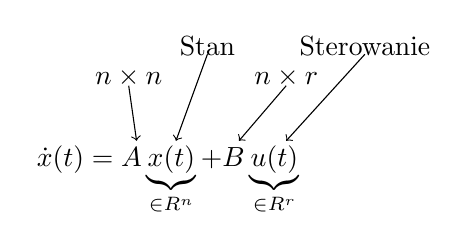
\begin{tikzpicture}
	\node at(0,0){$\dot{x}(t)=A\underbrace{x(t)}_{\in \mathbb{R}^n}+B\underbrace{u(t)}_{\in \mathbb{R}^r}$};
	\node at(-.5,1.3){{$n\times n$}};
	\node at(1.5,1.3){{$n\times r$}};
	\node at(.5,1.7){Stan};
	\node at(2.5,1.7){Sterowanie};

	\draw[->](-.5,1.2)--(-.4,.5);
	\draw[->](1.5,1.2)--(.9,.5);
	\draw[->](.5,1.6)--(.1,.5);
	\draw[->](2.5,1.6)--(1.5,.5);
\end{tikzpicture}
\end{figure}
\\
rozwiązanie:\\
$x(t)=e^{tA}x_0+\int^t_0e^{(t-r)A}Bu(r) \ dr$\\
\\
dla autonomicznych ($r=n=1, t\geqslant 0, u(t)\equiv 0$)\\
$x(t)=e^{tA}x_0$\\





\pagebreak
%###################                 1.1.1              #################################%
\subsection*{Zadanie 1.1.1} {\color{darkgray}
	Naszkicować rozwiazania równania rózniczkowego:\\
	$\dot{x}(t)=\alpha_ix(t)$\\
	dla $x(0)=1, t\geqslant 0$ przy czym $i=1,2,3$ zaś\\
	$\alpha_1=1,  \ \ \ \alpha_2=2, \ \ \ \alpha_3=-1$\\
}\lineh
\\\\
{\color{lightgray}
$\frac{dx}{dt}=\alpha_ix$\\
$\frac{dx}{x}=\alpha_idt$\\
całkowanie:\\
$\ln|x|=\alpha_i t+{c}$\\
}
$x=ce^{\alpha_it}$\\
$x(0)=c=1$\\
$x=e^{\alpha_it}$\\
\\
$x=e^t \ \vee \ x=e^{2t} \ \vee \ x=e^{-t}$\\
($t\geqslant 0$, więc tylko prawa strona)\\

\begin{figure}[!h]
\begin{tikzpicture}
	\draw [color=blue, thick]%(-3.0,0.02)--(-2.75,0.03)--(-2.5,0.04)--(-2.25,0.05)--(-2.0,0.06)--(-1.75,0.08)--(-1.5,0.11)--(-1.25,0.14)--(-1.0,0.18)--(-0.75,0.23)--(-0.5,0.3)--(-0.25,0.38)--
(0.0,0.5)--(0.25,0.64)--(0.5,0.82)--(0.75,1.05)--(1.0,1.35)--(1.25,1.74)--(1.5,2.24)--(1.75,2.87);
	\draw [color=blue, thick]%(-3.0,0.0)--(-2.75,0.0)--(-2.5,0.0)--(-2.25,0.0)--(-2.0,0.0)--(-1.75,0.01)--(-1.5,0.02)--(-1.25,0.04)--(-1.0,0.06)--(-0.75,0.11)--(-0.5,0.18)--(-0.25,0.3)--
(0.0,0.5)--(0.25,0.82)--(0.5,1.35)--(0.75,2.24)--(1.0,3.69);
	\draw [color=blue, thick]%(-2.0,3.69)--(-1.75,2.87)--(-1.5,2.24)--(-1.25,1.74)--(-1.0,1.35)--(-0.75,1.05)--(-0.5,0.82)--(-0.25,0.64)--
(0.0,0.5)--(0.25,0.38)--(0.5,0.3)--(0.75,0.23)--(1.0,0.18)--(1.25,0.14)--(1.5,0.11)--(1.75,0.08)--(2.0,0.06)--(2.25,0.05)--(2.5,0.04)--(2.75,0.03)--(3.0,0.02);


	\node at(2,3){$\alpha_1$};
	\node at(1.2,3.8){$\alpha_2$};
	\node at(3,.2){$\alpha_3$};


	\draw[thick][->](-3,0)--(3,0) node [right=3pt]{$t$};
	\draw[thick][->](0,-3)--(0,3) node [right=3pt]{$x$};



	\draw (-0.1,.5) -- (0.1,.5) node [left=3pt]{{1}};
	\draw (1,-0.1) -- (1,0.1) node [below=4pt]{{1}};
\end{tikzpicture}
\end{figure}



\pagebreak
%###################                 1.2.1              #################################%
\subsection*{Zadanie 1.2.1} {\color{darkgray}
	Naszkicować rozwiazania równania rózniczkowego:\\
	$\dot{x}(t)=\alpha_ix(t)$\\
	dla $x(0)=-1, t\geqslant 0$ przy czym $i=1,2,3$ zaś\\
	$\alpha_1=-1,  \ \ \ \alpha_2=-2, \ \ \ \alpha_3=1$\\
}\lineh
\\\\
$x=ce^{\alpha_it}$\\
$x(0)=c=-1$\\
$x=-e^{\alpha_it}$\\
\\
$x=-e^{-t} \ \vee \ x=-e^{-2t} \ \vee \ x=-e^{t}$\\
($t\geqslant 0$, więc tylko prawa strona)\\
\begin{figure}[!h]
\begin{tikzpicture}
\draw [color=blue, thick]%(-1.5,-2.24)--(-1.25,-1.74)--(-1.0,-1.35)--(-0.75,-1.05)--(-0.5,-0.82)--(-0.25,-0.64)--
(0.0,-0.5)--(0.25,-0.38)--(0.5,-0.3)--(0.75,-0.23)--(1.0,-0.18)--(1.25,-0.14)--(1.5,-0.11)--(1.75,-0.08)--(2.0,-0.06)--(2.25,-0.05)--(2.5,-0.04)--(2.75,-0.03)--(3.0,-0.02);
\draw [color=blue, thick]%(-0.75,-2.24)--(-0.62,-1.74)--(-0.5,-1.35)--(-0.37,-1.05)--(-0.25,-0.82)--(-0.12,-0.64)--
(0.0,-0.5)--(0.12,-0.38)--(0.25,-0.3)--(0.37,-0.23)--(0.5,-0.18)--(0.62,-0.14)--(0.75,-0.11)--(0.87,-0.08)--(1.0,-0.06)--(1.12,-0.05)--(1.25,-0.04)--(1.37,-0.03)--(1.5,-0.02)--(1.62,-0.01)--(1.75,-0.01)--(1.87,-0.01)--(2.0,0.0)--(2.12,0.0)--(2.25,0.0)--(2.37,0.0)--(2.5,0.0)--(2.62,0.0)--(2.75,0.0)--(2.87,0.0)--(3.0,0.0);\draw [color=blue, thick]%(-3.0,-0.02)--(-2.87,-0.02)--(-2.75,-0.03)--(-2.62,-0.03)--(-2.5,-0.04)--(-2.37,-0.04)--(-2.25,-0.05)--(-2.12,-0.05)--(-2.0,-0.06)--(-1.87,-0.07)--(-1.75,-0.08)--(-1.62,-0.09)--(-1.5,-0.11)--(-1.37,-0.12)--(-1.25,-0.14)--(-1.12,-0.16)--(-1.0,-0.18)--(-0.87,-0.2)--(-0.75,-0.23)--(-0.62,-0.26)--(-0.5,-0.3)--(-0.37,-0.34)--(-0.25,-0.38)--(-0.12,-0.44)--
(0.0,-0.5)--(0.12,-0.56)--(0.25,-0.64)--(0.37,-0.72)--(0.5,-0.82)--(0.62,-0.93)--(0.75,-1.05)--(0.87,-1.19)--(1.0,-1.35)--(1.12,-1.54)--(1.25,-1.74)--(1.37,-1.97)--(1.5,-2.24);

	\node at(1.5,-.4){$\alpha_1$};
	\node at(1.5,.2){$\alpha_2$};
	\node at(1.5,-2.5){$\alpha_3$};


	\draw[thick][->](-3,0)--(3,0) node [right=3pt]{$t$};
	\draw[thick][->](0,-3)--(0,3) node [right=3pt]{$x$};



	\draw (-0.1,.5) -- (0.1,.5) node [left=3pt]{{1}};
	\draw (1,-0.1) -- (1,0.1) node [below=4pt]{{1}};
\end{tikzpicture}
\end{figure}

\pagebreak
%###################                 1.3.1              #################################%
\subsection*{Zadanie 1.3.1} {\color{darkgray}
	Naszkicować rozwiazania równania rózniczkowego:\\
	$\dot{x}(t)=-x(t)+u_i$\\
	dla $x(0)=1, t\geqslant 0$ przy czym $i=1,2,3$ zaś\\
	$u_1=0,  \ \ \ u_2=1, \ \ \ u_3=2$\\
}\lineh
\\\\
$\frac{dx}{dt}=-x+u_i$\\
$\frac{dx}{-x+u_i}=dt$\\
całkowanie:\\
$-\ln|-x+u_i|=t+c$\\
$ce^{-t}=-x+u_i$\\
$x=u_i-ce^{-t}$\\
$x(0)=u_i-c=1\Rightarrow c=u_i-1$\\
$x=u_i-(u_i-1)e^{-t}=u_i(1-e^{-t})+e^{-t}$\\
\\
$x=e^{-t} \ \vee \ x=1 \ \vee \ x=2-e^{-t}$\\
($t\geqslant 0$, więc tylko prawa strona)\\

\begin{figure}[!h]
\begin{tikzpicture}
\draw [color=gray, dashed](0.0,1)--(3,1);
\draw [color=blue, thick]%(-2.0,3.69)--(-1.75,2.87)--(-1.5,2.24)--(-1.25,1.74)--(-1.0,1.35)--(-0.75,1.05)--(-0.5,0.82)--(-0.25,0.64)--
(0.0,0.5)--(0.25,0.38)--(0.5,0.3)--(0.75,0.23)--(1.0,0.18)--(1.25,0.14)--(1.5,0.11)--(1.75,0.08)--(2.0,0.06)--(2.25,0.05)--(2.5,0.04)--(2.75,0.03)--(3.0,0.02);
\draw [color=blue, thick](0.0,.5)--(3,.5);
\draw [color=blue, thick]%(-2.0,-2.69)--(-1.75,-1.87)--(-1.5,-1.24)--(-1.25,-0.74)--(-1.0,-0.35)--(-0.75,-0.05)--(-0.5,0.17)--(-0.25,0.35)--
(0.0,0.5)--(0.25,0.61)--(0.5,0.69)--(0.75,0.76)--(1.0,0.81)--(1.25,0.85)--(1.5,0.88)--(1.75,0.91)--(2.0,0.93)--(2.25,0.94)--(2.5,0.95)--(2.75,0.96)--(3.0,0.97);


	\node at(3.1,.2){$u_1$};
	\node at(3.3,.5){$u_2$};
	\node at(3.3,.9){$u_3$};


	\draw[thick][->](-3,0)--(3,0) node [right=3pt]{$t$};
	\draw[thick][->](0,-3)--(0,3) node [right=3pt]{$x$};



	\draw (-0.1,.5) -- (0.1,.5) node [left=3pt]{{1}};
	\draw (1,-0.1) -- (1,0.1) node [below=4pt]{{1}};
\end{tikzpicture}
\end{figure}


\pagebreak
%###################                 1.4.1              #################################%
\subsection*{Zadanie 1.4.1} {\color{darkgray}
	Naszkicować rozwiazania równania rózniczkowego:\\
	$\dot{x}(t)=-x(t)+1$\\
	dla $x(0)=x_i, t\geqslant 0$ przy czym $i=1,2,3$ zaś\\
	$x_1=0,  \ \ \ x_2=1, \ \ \ x_3=2$\\
}\lineh
\\\\
$\frac{dx}{dt}=-x+1$\\
$-\ln|-x+1|=t+c$\\
$ce^{-t}=-x+1$\\
$x=1-ce^{-t}$\\
$x(0)=1-c=x_i\Rightarrow c=1-x_i$\\
$x=1-(1-x_i)e^{-t}$\\
\\
$x=1-e^{-t} \ \vee \ x=1 \ \vee \ x=1+e^{-t}$\\
($t\geqslant 0$, więc tylko prawa strona)\\
\begin{figure}[!h]
\begin{tikzpicture}
\draw [color=blue, thick]%(-1.75,-2.37)--(-1.5,-1.74)--(-1.25,-1.24)--(-1.0,-0.85)--(-0.75,-0.55)--(-0.5,-0.32)--(-0.25,-0.14)--
(0.0,0.0)--(0.25,0.11)--(0.5,0.19)--(0.75,0.26)--(1.0,0.31)--(1.25,0.35)--(1.5,0.38)--(1.75,0.41)--(2.0,0.43)--(2.25,0.44)--(2.5,0.45)--(2.75,0.46)--(3.0,0.47);
\draw [color=blue, thick](0.0,.5)--(3,.5);
\draw [color=blue, thick]%(-1.75,3.37)--(-1.5,2.74)--(-1.25,2.24)--(-1.0,1.85)--(-0.75,1.55)--(-0.5,1.32)--(-0.25,1.14)--
(0.0,1.0)--(0.25,0.88)--(0.5,0.8)--(0.75,0.73)--(1.0,0.68)--(1.25,0.64)--(1.5,0.61)--(1.75,0.58)--(2.0,0.56)--(2.25,0.55)--(2.5,0.54)--(2.75,0.53)--(3.0,0.52);



	\node at(-.3,-.3){$x_1$};
	\node at(-.5,.5){$x_2$};
	\node at(-.3,1){$x_3$};


	\draw[thick][->](-3,0)--(3,0) node [right=3pt]{$t$};
	\draw[thick][->](0,-3)--(0,3) node [right=3pt]{$x$};



	\draw (-0.1,.5) -- (0.1,.5) node [left=3pt]{{1}};
	\draw (1,-0.1) -- (1,0.1) node [below=4pt]{{1}};
\end{tikzpicture}
\end{figure}


\pagebreak
%###################                 1.5.1              #################################%
\subsection*{Zadanie 1.5.1} {\color{darkgray}
	Dany jest obwód elektryczny jak na rysunku poniżej.\\
	\begin{figure}[!h]
	\begin{tikzpicture}
	\draw[scale=0.8, transform shape]
	(0,0) to[american current source,l=$u(t)$] 
	(0,3) to [european resistor,l=R,i=$i_c$] (3,3) to [C,l=C] (3,0) -- (0,0);
	\draw[->] (3.5,0.5) -- (3.5,2) node[right,pos=.5] {$x_1=U_c$};

	\draw (1,1) arc (240:-50:.3 and .3);
	\draw[->] (1.35,1.04)  -- (1.25,.94) ;

	\node at (6.5,2) {$R=100[K\Omega] $};
	\node at (6.85,1.5) {$U_c(0)=-1.72[V]$};
	\node at (6.3,1) {$C=1 [\mu F]$};
	\end{tikzpicture}	
	\end{figure}
\\
Źródło napięcia przez jedną sekundę podawało napięcie $1 [V]$, a następnie przestało podawać dalej napięcie (przyjąć $0 [V]$). Zamodelować obwód w postaci równania różniczkowego, wyliczyć wartość napięcia w chwili $T = 2 [s]$ i naszkicować przebieg napięcia w funkcji czasu.\\
}\lineh
\\\\
$i(t)=c\cdot \dot{x}_1(t)$\\
$u-Ri_c-x_1=0$\\
$u(t)-RCx_1'(t)-x_1(t)=0$\\
$ \begin{array}{ll}
1^\circ \ \ t\in<0,1> \ \ \boxed{u(t)=1}&2^\circ \ \ t>0 \ \ \boxed{u(t)=0}\\
1-RCx_1'(t)-x_1(t)=0&x_2'(t)=-\frac{x_2(t)}{RC}\\
x_1'(t)=-\frac{x_1(t)}{RC}+\frac{1}{RC}&\frac{dx_2}{dt}=-\frac{1}{RC}x_2\\
\frac{dx_1}{dt}=\frac{1}{RC}(1-x_1)&\frac{dx_2}{x_2}=-\frac{1}{RC}dt\\
\frac{dx_1}{1-x_1}=\frac{1}{RC}dt&\ln|x_2|=-\frac{t}{RC}+k\\
-\ln|1-x_1|=\frac{1}{RC}t+k&ke^{-\frac{t}{RC}}=x_2\\
ke^{-\frac{t}{RC}}=1-x_1&x_2(0)=x_1(1)\\
x_1=1-ke^{-\frac{t}{RC}}&x_2(0)=k=x_1(1)\\
x_1(0)=u_c=-1.72=1-k \Rightarrow k=2.72&x_2(2)=x_1(1)e^{-\frac{2}{RC}}\\
x_1(1)=1-2.72e^{-\frac{1}{RC}} \approx 0.000632&x_2(2)=-0.0000855


\end{array}$\\








\pagebreak
%###################                 1.6.1              #################################%
\subsection*{Zadanie 1.6.1} {\color{darkgray}
	Dane jest równanie różniczkowe\\
	$\dot{x}(t)=-2x(t)+u(t)$\\
	gdzie $x(0)=1, t\geqslant 0$. Znaleźć takie sterowanie $u(t)$, że $x(t)=e^{-t}$ dla $t \geqslant 0$.\\
}\lineh
\\\\
$x(t)=e^{-t}$\\
$x'(t)=-e^{-t}$\\
przyrównujemy $\dot{x}(t)$\\
$-e^{-t}=-2e^{-t}+u(t) \Rightarrow \boxed{u(t)=e^{-t}}$\\

\pagebreak
%###################                 1.7.1              #################################%
\subsection*{Zadanie 1.7.1} {\color{darkgray}
	Zamodelować poniższy obwód elektryczny za pomocą równania różniczkowego\\
	\begin{figure}[!h]
	\begin{tikzpicture}
	\draw[transform shape,thick]
(0,2) to  [C,l=C]  (0,-2) to [european resistor,l={\tiny$\frac{1}{2}R$}] (2,0) to [european resistor,l={\tiny$\frac{1}{3}R$}](0,2) to [european resistor,l={\tiny$\frac{1}{2}R$}](-2,0) to [european resistor,l={\tiny$\frac{1}{2}R$}](0,-2) to [european resistor,l={\tiny$\frac{1}{3}R$}](2,-4) to [european resistor,l={\tiny$2R$}](4,-2) to [european resistor,l={\tiny$3R$}](2,0) to [european resistor,l={\tiny$\frac{1}{2}R$}](4,2) to [european resistor,l={\tiny$2R$}](2,4) to [european resistor,l={\tiny$3R$}](0,2) to [european resistor,l={\tiny$3R$}](-2,4) to [european resistor,l={\tiny$2R$}](-4,2) to [european resistor,l={\tiny$\frac{1}{3}R$}](-2,0) to [european resistor,l={\tiny$\frac{1}{3}R$}](-4,-2) to [european resistor,l={\tiny$2R$}](-2,-4) to [european resistor,l={\tiny$3R$}](0,-2);

	\fill[fill=black](-2,0) circle(3pt);
	\fill[fill=black](2,0) circle(3pt);
	\fill[fill=black](0,2) circle(3pt);
	\fill[fill=black](0,-2) circle(3pt);
	\end{tikzpicture}	
	\end{figure}
\\
Przy czym $R=4.7k\Omega$ zaś $C=2\mu F$.\\
}\lineh
\\\\
	\begin{figure}[!h]
	\begin{tikzpicture}
	\draw[transform shape,thick]
(0,2) to  [C,l=C]  (0,-2) to [european resistor,l={\tiny$\frac{1}{2}R$}] (2,0) to [european resistor,l={\tiny$\frac{1}{3}R$}](0,2) to [european resistor,l={\tiny$\frac{1}{2}R$}](-2,0) to [european resistor,l={\tiny$\frac{1}{2}R$}] (0,-2) to (1,-3) to [european resistor,l={\tiny$5\frac{1}{3}R$}](3,-1) to (2,0) to (3,1) to [european resistor,l={\tiny$5\frac{1}{2}R$}](1,3) to (0,2) to (-1,3) to [european resistor,l={\tiny$5\frac{1}{3}R$}](-3,1) to (-2,0) to (-3,-1) to [european resistor,l={\tiny$5\frac{1}{3}R$}](-1,-3) to (0,-2);

	\fill[fill=black](-2,0) circle(3pt);
	\fill[fill=black](2,0) circle(3pt);
	\fill[fill=black](0,2) circle(3pt);
	\fill[fill=black](0,-2) circle(3pt);
	\end{tikzpicture}	
\hfill
	\begin{tikzpicture}
	\draw[transform shape,thick]
(0,2) to  [C,l=C]  (0,-2) to [european resistor,l={\tiny$\frac{16}{35}R$}] (2,0) to [european resistor,l={\tiny$\frac{11}{35}R$}](0,2) to [european resistor,l={\tiny$\frac{16}{35}R$}](-2,0) to [european resistor,l={\tiny$\frac{16}{35}R$}] (0,-2);

	\fill[fill=black](0,2) circle(3pt);
	\fill[fill=black](0,-2) circle(3pt);
	\end{tikzpicture}	
\hfill
	\begin{tikzpicture}
	\draw[transform shape,thick]
(0,1) to  [C,l=C]  (0,-1) to(2,-1)to [european resistor,l={\tiny$\frac{32}{35}R$}] (2,1) to (0,1) to (-2,1)to [european resistor,l={\tiny$\frac{27}{35}R$}](-2,-1) to  (0,-1);

	\fill[fill=black](0,1) circle(3pt);
	\fill[fill=black](0,-1) circle(3pt);
	\end{tikzpicture}	
\hfill
	\begin{tikzpicture}
	\draw[transform shape,thick]
(0,1) to  [C,l=C]  (0,-1) to(2,-1)to [european resistor,l={\tiny$\frac{864}{2065}R$}] (2,1) to (0,1) ;

	\end{tikzpicture}	
	\end{figure}
\\
$u(t)=RC\dot{x}(t)+x(t)$\\
$x'(t)=\frac{u(t)}{RC}-\frac{x}{RC}$\\
$u(t)=0$\\
$x'(t)=-\frac{x}{RC}$\\
$\boxed{x'(t)=-\frac{x}{\frac{864}{2065}\cdot R\cdot C}}$\\
$\boxed{\begin{aligned}\frac{dx}{dt}=-\frac{x}{RC}\\
\ln |x|=-\frac{t}{RC}+k\\
ke^{-\frac{t}{RC}}=x\end{aligned}}$\\


\pagebreak
%###################                 1.8.1              #################################%
\subsection*{Zadanie 1.8.1} {\color{darkgray}
	Dane jest równanie różniczkowe\\
	$\dot{x}(t)=-2x(t)+3$\\
	gdzie $x(0)=-1, t\geqslant 0$. Po jakim czasie $t_k$ zachodzi $x(t_k)=2$.\\
}\lineh
\\\\
$\frac{dx}{dt}=-2x(t)+3$\\
$\frac{dx}{-2x+3}=dt$\\
$\int \frac{1}{-2x+3} dx = \left|\begin{array}{c}u=-2x+3 \\du=-2dx\end{array}\right|=-\frac 12 \ln |-2x+3|=t+c$\\
$ce^{-2t}=-2x+3$\\
$x=\frac{3-ce^{-2t}}{2}$\\
$x(0)=\frac{3-c}{2}=-1 \Rightarrow c=5$\\
$x=\frac{3-5e^{-2t}}{2}$\\
$x(t_k)=2=\frac{3-5e^{-2t_k}}{2}$\\
$4=3-5e^{-2t_k} \Rightarrow e^{-2t_k}=-\frac 15 \ \ \boxed{\text{Sprzeczność}}$\\





\pagebreak
%###################                 1.9.1              #################################%
\subsection*{Zadanie 1.9.1} {\color{darkgray}
	Rozwiązanie równania różniczkowego\\
	$\dot{x}(t)=-100x(t)+2\sin(t)$\\
	gdzie $x(0)=2, t\geqslant 0$ ma postać\\
	$x(t)=ae^{-100t}+A\sin(t+\varphi)$\\
	Obliczyć $A$ i $\varphi$.\\
}\lineh
\\\\
Pochodna równania (2):\\
$\dot{x}(t) = -100ae^{-100t} + A cos(t + \varphi) $\\
Z równań (1) i (3):\\
$-100ae^{-100t} + A cos(t + \varphi) = -100x(t) + 2sin(t)$\\
Założenie, żeby ułatwić życie: $t = 0$\\
$ \left \{ {{-100a + A cos(\varphi) = -200} \atop {a + A sin(\varphi) = 2} \quad /*(-100)} \right. $\\
$ \left \{ {{-100a + A cos(\varphi) = -200} \atop {-100a -100A sin(\varphi) = -200}} \right. $\\
$A cos(\varphi) = -100A sin(\varphi)$\\
$\frac{sin(\varphi)}{cos(\varphi)} = tg(\varphi) = -\frac{1}{100}$\\
$\varphi = arctg(-\frac{1}{100})$\\
\\
Dalej chyba logiczne:\\
$x(0) = 2 = a + A sin(\varphi)$\\
$A sin(\varphi) = 2-a$\\
$A = \frac{2-a}{sin(arctg(-\frac{1}{100}))}$\\
\lineh
\\\\
{\color{red} Drugie rozwiązanie}\\
$x(0)=a+A\sin \varphi =2 \Rightarrow \boxed{A=\frac{2-a}{\sin \varphi}}$\\
$\frac{dx}{dt}+100x=2\sin t$\\
$\frac{dx}{dt}+100x=0$\\
$\ln|x|=-100t+c$\\
$c(t)e^{-100t}=x$\\
$c'e^{-100t}-\cancel{100ce^{-100t}}=-\cancel{100ce^{-100t}}+2\sin t$\\
$c'=2\sin t e^{100t}$\\
$\int \sin t e^{100t}=\left|\begin{array}{cc}\sin t & \cos t \\ e^{100t} & \frac{1}{100}e^{100t}\end{array}\right|=\frac{1}{100}\sin t e^{100t}-\frac{1}{100} \int \cos t e^{100t}=\left|\begin{array}{cc}\cos t & \sin t \\ e^{100t} & \frac{1}{100}e^{100t}\end{array}\right|=$\\
$=\frac{1}{100}\sin t e^{100t}-\frac{1}{100^2}\cos t e^{100t}-\frac{1}{100} \int \sin t e^{100t} \Rightarrow \int \sin t e^{100t} dt = \boxed{\frac{100\sin t - \cos t}{1001}e^{100t}+c}$\\
$\boxed{x=Ke^{-100t}+2\cdot\frac{100\sin t - \cos t}{10001}}$\\
$x=Ke^{-100t}+\frac{200\sin t -2\cos t}{10001}$\\
$x(0)=K-\frac{2}{10001}=2 \Rightarrow K=\frac{20004}{10001}$\\
$ae^{-100t}+A\sin(t+\varphi)=Ke^{-100t}+\frac{200\sin t - 2 \cos t}{10001}$\\
$a=K$\\
$A=\frac{2-a}{\sin \varphi}=\frac{2-\frac{20004}{10001}}{\sin \varphi}=\frac{-2}{1000t\sin\varphi}$\\
$A(\sin t \cos \varphi + \sin \varphi \cos t)=\frac{200\sin t}{10001}-\frac{2\cos t}{10001}$\\
$\cancel{\sin t}\text{ctg}\varphi+\cancel{\cos t}=-100\cancel{\sin t}+\cancel{\cos t}$\\
$\text{ctg}\varphi= -100$\\
$\text{tg}\varphi=\frac{-1}{100} \Rightarrow \boxed{\text{arctg}(\frac{-1}{100})=\varphi}$\\


\pagebreak
%###################                 1.10.1              #################################%
\subsection*{Zadanie 1.10.1} {\color{darkgray}
	Dane jest równanie różniczkowe\\
	$\dot{x}(t)=-x(t)+u(t)$\\
	gdzie $x(0)=0, t\geqslant 0$\\
	zaś sterowanie ma postać sygnału PWM o amplitudzie 15, okresie 1s i współczynniku wypełnienia $\theta \in (0,1]$, tzn.\\
	$u(t)=\left\{ \begin{array}{ccl} 15 &\text{dla} & t\in [n,n+\theta] \\ 0 & \text{dla} &t \in(n+\theta, n+1)\end{array}\right.$\\
	Wiedząc, że $x(3)=1$ obliczyć $\theta$.\\
}\lineh
\\\\
$x(t)=\underbrace{e^{tA}x(0)}_{=0}+\int^t_0 e^{(t-\tau)A}Bu(\tau)\ d\tau$\\
$x(t)=\int^t_0 e^{-t+\tau}u \ d\tau$\\
$x(3)=ue^{-3}\int_0^3e^\tau \ \ d\tau=15e^{-3}(e^\theta-1+e^{1+\theta}-e+e^{2+\theta}-e^2)=15e^{-3}(e^\theta(1+e+e^2)-(1+e+e^2))=15e^{-3}((e^\theta-1)(1+e+e^2))=\boxed{1}$\\
$\frac{e^3}{15(1+e+e^2)}+1=e^\theta \Rightarrow \boxed{\theta=\ln(1+\frac{e^3}{15(1+e+e^2)})}$\\

